\section{Continuous Random Variables}
\subsection{Basic definitions}
Recall that for a probability space $(\Omega,\mathscr F,\mathbb P)$, a random variable is a function $X:\Omega\to\mathbb R$ such that $\{X\le x\}=\{\omega\in\Omega:X(\omega)\le x\}\in\mathscr F$. 

\begin{definition}[Probability distribution function]
    The \textbf{probability distribution function} $ F:\bbR\to [0,1] $ is defined by $F(x)=\mathbb P(X\le x)$.
\end{definition}

\begin{proposition}\
    \begin{enumerate}
        \item $x\le y\implies F(x)\le F(y)$.
        \item $\forall a<b,\mathbb P(a<X\le b)=F(b)-F(a)$.
        \item $F$ is right continuous and the left limits always exist as well. Also,
        $$F(x-)=\mathbb{P}(X<x)\le F(x).$$
        \item $\displaystyle \lim_{x\to-\infty}F(x)=0,\lim_{x\to\infty}F(x)=1.$
    \end{enumerate}
\end{proposition}
\begin{proof}\
    \begin{enumerate}
        \item $ \{X\le x\} \subseteq \{X\le Y\} $.
        \item $ \mathbb{P}(a<x\le b)=\mathbb{P}(\{X>a\}\cap \{X\le b\})=\mathbb{P}(X\le b)-\mathbb{P}(\{X\le b\}\cap \{X\le a\})=\mathbb{P}(X\le b)-\mathbb{P}(X\le a)=F(b)-F(a) $.
        \item It suffices to prove $ \lim_{n \to \infty} F(x+\frac{1}{n})=F(x) $. Define $ A_n=\{x<X\le x+\frac{1}{n}\} $. Then $(A_n)$ are decreasing and $ \cap A_n = \varnothing $. But $ \mathbb{P}(A_n)=F(x+\frac{1}{n})-F(x)\to 0 $, so this proves right continuity. 

        Left limits exist since $F$ is increasing. Note that $ F(x-)=\lim_{n \to \infty} F(x-\frac{1}{n}) $ and that $ F(x-\frac{1}{n})=\mathbb{P}(X\le x-\frac{1}{n}) $. Consider $ B_n=\{X\le x-\frac{1}{n}\} $. Then $ (B_n) \nearrow, \cup B_n=\{X<x\} $, and $ \mathbb{P}(B_n)\to\mathbb{P}(X<x)\to F(x-)\le F(x) $.
        \item This one is easy.
    \end{enumerate}
\end{proof}

For example, $F$ of a discrete random variable might look like this:
\begin{center}
  \begin{tikzpicture}
    \draw [->] (0, 0) -- (3, 0);
    \draw [->] (0, 0) -- (0, 2) node [above] {$F$};
    \draw (0,0.5) -- (1,0.5);
    \node [dot=3.5pt] at (0,0.5) {};
    \draw [dashed] (1,0.5) -- (1,1);
    \node [dot=3.5pt] at (1,1) {};
    \node at (1,0.5) {$ \circ $};
    \draw (1,1) -- (2,1);
    \draw [dashed] (2,1) -- (2,1.5);
    \node [dot=3.5pt] at (2,1.5) {};
    \node at (2,1) {$ \circ $};
    \draw (2,1.5) -- (3,1.5);
    \node at (3,1.5) {$ \circ $};
  \end{tikzpicture}
\end{center}
It is indeed right continuous with left limits.

\begin{definition}[Continuous random variable]
    $X$ is a \textbf{continuous random variable} if $F$ is continuous, which means that $ F(x)=F(x-),\forall x \Longrightarrow \mathbb{P}(X\le x)=\mathbb{P}(X<x),\forall x $. In other words, $ \mathbb{P}(X=x)=0, \forall x\in \mathbb{R}  $.
    \begin{center}
        \begin{tikzpicture}
          \draw [->] (0, 0) -- (3, 0);
          \draw [->] (0, 0) -- (0, 2) node [above] {$F$};
          \draw (0, 0) parabola (2.5, 1.5);
        \end{tikzpicture}
    \end{center}
\end{definition}
\begin{definition}[Absolutely continous]
    $F$ is called \textbf{absolutely continous} if $F$ is not only continuous but also differentiable. 
\end{definition}
In this course we will further restrict to absolutely continuous $F$.

\subsection{Probability density function}

\begin{definition}[Probability density function]
    Set $F'(x)=f(x)$. We call $f$ the \textbf{probability density function} of $X$. 
\end{definition}

\begin{proposition}[Properties of $f$]\
    \begin{enumerate}
        \item$f(x)\ge 0$.
        \item $ \int_{-\infty}^x f(y)\,\mathrm dy=F(x). $ In particular, $ \int_{-\infty}^\infty f(y)\,\mathrm dy=1. $
    \end{enumerate}
\end{proposition}
Intuitively, for $\Delta x$ small, we have
\[
    \mathbb P(x<X\le x+\Delta x)=\int_x^{x+\Delta x}f(y)\,\mathrm dy\approx f(x)\Delta x,
\]
which is like approximating a continuous random variable by the probability density function of a discrete random variable. 

More generally, for any set $ S \subseteq \mathbb{R}  $, 
\[
    \mathbb{P}(x\in S) = \int_{S} f(x) \,\mathrm{d}x.
\]

\begin{center}
    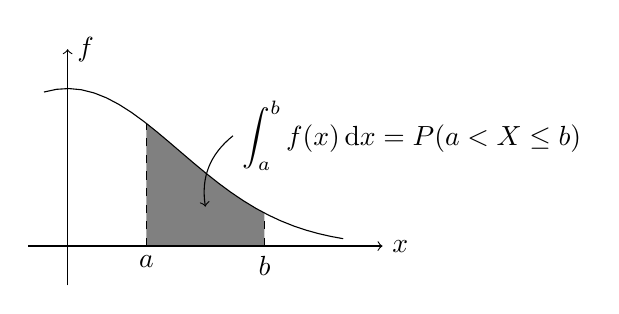
\begin{tikzpicture}
        \fill [gray, domain=1:2.5, variable=\x]
        (1, 0)
        -- plot (\x, {2 * exp(-\x * \x / 4)})
        -- (2.5, 0)
        -- cycle;
        \draw [->] (-0.5,0) -- (4,0) node [right] {$ x $};
        \draw [->] (0,-0.5) -- (0,2.5) node [right] {$ f $};
        \draw [domain=-0.3:3.5, variable=\x] plot (\x, {2 * exp(-\x * \x / 4)});
        \node [below] at (1,0) {$a$};
        \node [below] at (2.5,0) {$b$};
        \draw [->, bend right] (2.1, 1.4) to (1.75, 0.5);
        \node [right] at (2.1, 1.4) {$\displaystyle \int_{a}^{b} f(x) \,\mathrm{d}x = \mathbb{P}(a<X\le b)$};
        \draw [dashed] (1,0) -- (1,1.56);
        \draw [dashed] (2.5,0) -- (2.5,0.42);
    \end{tikzpicture}
\end{center}

\subsection{Expectation and variance}
\begin{definition}[Expectation of positive continuous r.v.]
    Let $X\ge 0$ with density $f$. Define its \textbf{expectation} as 
    \[
        \bbE[X] = \int_{0}^{\infty} xf(x) \,\mathrm{d}x.
    \]
\end{definition}\
\begin{note}
    Suppose $g\ge 0$. Then for any variable $X$,
    \[
        \bbE[g(X)]= \int_{-\infty}^{\infty} g(x)f(x) \,\mathrm{d}x.
    \]
\end{note}
\begin{definition}[Expectation of general continuous r.v.]
    Let $X$ be a general r.v. Define $ X_+=\max \{X,0\},X_-=\max \{-X,0\} $. If at least one of $ \bbE[X_+],\bbE[X_-] $ is finite, then define 
    \[
        \bbE[X]=\bbE[X_+]-\bbE[X_-] = \int_{-\infty}^{\infty} xf(x) \,\mathrm{d}x.
    \]
\end{definition}
\begin{note}
    The last equality comes from 
    \[
        \bbE[X_+] = \int_{0}^{\infty} xf(x) \,\mathrm{d}x,\quad \bbE[X_-]=\int_{-\infty}^{0} xf(x) \,\mathrm{d}x.
    \]
    It is easy to check that the expectation is a \textit{linear} function.
\end{note}

\begin{proposition}
    Let $X\ge 0$. Then 
    \[
        \bbE[X] = \int_{0}^{\infty} \mathbb{P}(X\ge x) \,\mathrm{d}x.
    \]
\end{proposition}
\begin{proof}
    \begin{align*}
        \bbE[X]&= \int_{0}^{\infty} xf(x) \,\mathrm{d}x=\int_{0}^{\infty} \left( \int_{0}^{x}  \,\mathrm{d}y \right)f(x) \,\mathrm{d}x\\ 
        \text{(Check!)}&= \int_{0}^{\infty} \int_{y}^{\infty} f(x) \,\mathrm{d}x \,\mathrm{d}y = \int_{0}^{\infty} (1-F(y)) \,\mathrm{d}y\\ 
        &= \int_{0}^{\infty} \mathbb{P}(X\ge y) \,\mathrm{d}y.\qedhere
    \end{align*}
\end{proof}
\begin{proof}[Alternatively,]
    note that $ \forall \omega, X(\omega)=\int_{0}^{\infty} 1(X(\omega)\ge x) \,\mathrm{d}x $. Taking expectation we get 
    \begin{align*}
        \bbE[X] &= \bbE\left[ \sum_{\omega}\int_{0}^{\infty} 1(X(\omega)\ge x) \,\mathrm{d}x \right] = \bbE\left[ \int_{0}^{\infty} 1(X\ge x) \,\mathrm{d}x \right]\\
        &= \int_{0}^{\infty} \bbE[1(X(\omega)\ge x)] \,\mathrm{d}x = \int_{0}^{\infty} \mathbb{P}(X\ge x) \,\mathrm{d}x.\qedhere
    \end{align*}
\end{proof}
\begin{remark}
    The second proof is not rigorous since we did not justify interchanging $ \bbE $ and $ \int $.
\end{remark}

\begin{definition}[Variance]
    The \textbf{variance} of a continuous random variable is
    \[
        \var(X) = \bbE[(X-\bbE[X])^2] = \bbE[X^2]-(\bbE[X])^2.
    \]
\end{definition}

\subsection{Examples of continuous r.v.s}
\begin{example}[Uniform distribution]
    Let $a,b\in \bbR$ such that $a<b$. Define the density as 
\[
    f(x) = \begin{cases}
    \frac{1}{b-a} &\text{if }x\in [a,b]\\
    0 &\text{otherwise}\\
    \end{cases} 
\]
Then $X$ is called a \textbf{uniform} distribution and we write $ X \sim U[a,b] $, and the pdf is 
\[
    F(x)=\mathbb P(X\le x)=\int_{-\infty}^xf(y)\,\mathrm dy=\begin{cases}
        0&\text{if $x<a$}\\
        \frac{x-a}{b-a}&\text{if $x\in [a,b]$}\\
        1&\text{if $x>b$}
    \end{cases},
\]
and $ \bbE[X] $ is 
\[
    \mathbb E[X]=\int_{-\infty }^{\infty }xf(x)\,\mathrm dx=\int_a^bxf(x)\,\mathrm dx=\frac{a+b}{2}
\]
\end{example}

\begin{example}[Exponential distribution]
    The density is $ f(x)=\lambda e^{-\lambda x} $ where $ \lambda,x>0 $. Write $ X \sim \operatorname{Exp}(\lambda) $. Here 
    \[
        F(x)=\int_0^x\lambda e^{-\lambda y}\,\mathrm dy=1-e^{-\lambda x},.\quad \bbE[X]=\int_{0}^{\infty} \lambda x e^{-\lambda x} \,\mathrm{d}x=\frac{1}{\lambda}.
    \]
    \paragraph{Exponential as a limit of geometrics.} Let $T\sim\operatorname{Exp}(\lambda)$ and $T_n=\lfloor nT\rfloor$, so
    \[
        \mathbb P(T_n\ge k)=\mathbb P(T\ge k/n)=e^{-k\lambda/n}=(e^{-\lambda/n})^k,
    \]
    so $T_n$ is distributed geometrically with parameter $p_n=1-e^{-\lambda/n}$, so as $n\to\infty$, we have $p_n\sim \lambda/n$ and $T_n/n\to T$. So exponential is the limit of a rescaled geometric.
\end{example}

\begin{proposition}
    The exponential random variable is \emph{memoryless}, i.e.
    \[
        \bbP(T > t+s \mid T>s) = \bbP(T>t).
    \]
\end{proposition}
We have something stronger:
\begin{proposition}
    Let $ T $ be a positive continous r.v. not identically $0$ or $ \infty $ with density $f$. Then $T$ is memoryless if and only if $T$ is exponential.
\end{proposition}
\begin{proof}
    $ (\Leftarrow) $ is justified by proposition 3.4. $ (\Rightarrow ) $: Suppose $ \forall s,t,\ \mathbb{P}(T>t+s)=\mathbb{P}(T>s)\mathbb{P}(T>t) $. Set $ g(t)=\mathbb{P}(T>t) $. We want to show $ g(t)=e^{-\lambda t} $ for some $ \lambda>0 $. Note that $ \forall s,t>0,\ g(t+s)=g(t)g(s) $, and 
    \[
        \forall t\ge 0, \forall m\in \mathbb{N},\ g(mt)=(g(t))^m \Longrightarrow g(m)=g(1)^m.
    \]
    Furthermore, 
    \[
        \forall m,n\in \mathbb{N},\ g\left( \frac{m}{n} \right)^n=g(m) \Longrightarrow g\left( \frac{m}{n} \right)= g(m)^{1/n}=g(1)^{m/n}.
    \]
    Now $ g(1)=\mathbb{P}(T>1)\in (0,1) $, as $T$ would be identically $0$ or $ \infty $ otherwise. Set $ \lambda=-\log \mathbb{P}(T>1)>0 $. So we have proved that 
    \[
        \forall t\in \mathbb{Q}_+,\ g(t)=\mathbb{P}(T>t)=e^{-\lambda t}.
    \]
    Let $ t\in \mathbb{R}_+ $. Then $ \forall \epsilon,\ \exists r,s\in \mathbb{Q} $ such that $ r\le t\le s $ and $ |r-s|<\epsilon $. Now
    \[
        e^{-\lambda s}=\mathbb{P}(T>s)\le \mathbb{P}(T>t)\le \mathbb{P}(T>r) = e^{-\lambda r}.
    \]
    Since it holds for all $ \epsilon $, we must have $ \mathbb{P}(T>t)=e^{-\lambda t} $, as claimed.
\end{proof}

\begin{theorem}
    Let $X$ be a continuous random variable with density $f$.
    Let $g$ be a continuous, strictly monotone function with $g^{-1}$ differentiable.
    Then $g(X)$ is a continuous random variable with density
    \[
        f(g^{-1}(x))\left| \frac{\mathrm{d}}{\mathrm{d}x}g^{-1}(x) \right|. 
    \]
\end{theorem}
\begin{proof}
    First assume that $g$ is strictly increasing, then $\mathbb P(g(X)\le x)=\mathbb P(X\le g^{-1}(x))=F(g^{-1}(x))$, so the density of $g(X)$ would be
    $$\frac{\mathrm d}{\mathrm dx}F(g^{-1}(x))=f(g^{-1}(x))\frac{\mathrm dg^{-1}(x)}{\mathrm dx}=f(g^{-1}(x))\left|\frac{\mathrm dg^{-1}(x)}{\mathrm dx}\right|.$$
    As for $g$ strictly decreasing, $\mathbb P(g(X)\le x)=\mathbb P(X\ge g^{-1}(x))=1-F(g^{-1}(x))$, so the density is
    $$\frac{\mathrm d}{\mathrm dx}(1-F(g^{-1}(x)))=-f(g^{-1}(x))\frac{\mathrm dg^{-1}(x)}{\mathrm dx}=f(g^{-1}(x))\left|\frac{\mathrm dg^{-1}(x)}{\mathrm dx}\right|,$$
    as claimed.
\end{proof}
\begin{example}[Normal distribution]
    For $\mu\in\mathbb R,\sigma>0$, define $ f: \mathbb{R}\to \mathbb{R} $ by
    \[
        f(x) = \frac{1}{\sqrt{2\pi\sigma^2}}\exp\left(-\frac{(x - \mu)^2}{2\sigma^2}\right).
    \]
    \begin{center}
        \begin{tikzpicture}[yscale=1.5]
          \draw (-3, 0) -- (3, 0);
          \draw (0, 1.3) -- (0, 0) node [below] {$\mu$};
          \draw [domain=-3:3,samples=50, blue] plot (\x, {exp(-\x * \x)});
        \end{tikzpicture}
    \end{center}
    \begin{proof}[Check that $f$ is a density]
        Indeed, 
        \begin{align*}
            \int_{-\infty}^{\infty} f(x) \,\mathrm{d}x &= \int_{-\infty}^{\infty} \frac{1}{\sqrt{2\pi\sigma^2}}\exp\left(-\frac{(x - \mu)^2}{2\sigma^2}\right) \,\mathrm{d}x\\ 
            &= \int_{-\infty}^{\infty} \frac{1}{\sqrt{2\pi}}\exp \left( -\frac{u^2}{2} \right)\dd u\\ 
            &= 2 \int_{0}^{\infty} \frac{1}{\sqrt{2\pi}} \exp \left( -\frac{u^2}{2} \right)\dd u=:I.
        \end{align*}
        Then
        \begin{align*}
          I^2 &= \frac{\pi}{2} \int_{0}^{\infty} \int_{0}^{\infty} \exp \left( -\frac{u^2+v^2}{2} \right) \,\mathrm{d}u\,\mathrm{d}v\\ 
          &= \frac{\pi}{2}\int_0^\infty \int_0^{\pi/2}re^{-r^2/2}\dd r\dd \theta=1\\ 
          \Longrightarrow I&=1.\qedhere
        \end{align*}
    \end{proof}
    \begin{proposition}
        $\bbE[X] = \mu$.
    \end{proposition}
    \begin{proof}
    \begin{align*}
    \bbE[X] &= \frac{1}{\sqrt{2\pi}\sigma} \int_{-\infty}^\infty x e^{-(x - \mu)^2/2\sigma^2}\dd x\\
    &= \frac{1}{\sqrt{2\pi} \sigma}\int_{-\infty}^\infty (x - \mu)e^{-(x - \mu)^2/2\sigma^2}\dd x + \frac{1}{\sqrt{2\pi}\sigma}\int_{-\infty}^\infty \mu e^{-(x - \mu)^2/2\sigma^2}\dd x.
    \end{align*}
    The first term is antisymmetric about $\mu$ and gives $0$. The second is just $\mu$ times the integral we did above. So we get $\mu$.
    \end{proof}
    \begin{proposition}
    $\var(X) = \sigma^2$.
    \end{proposition}
    \begin{proof}
    We have $\var (X) = \bbE[X^2] - (\bbE[X])^2$. Substitute $Z = \frac{X - \mu}{\sigma}$. Then $\bbE[Z] = 0$, $\bbE[Z^2] = \frac{1}{\sigma^2}\bbE[X^2]$. Then
    \begin{align*}
        \var(Z) &= \frac{1}{\sqrt{2\pi}} \int_{-\infty}^\infty z^2 e^{-z^2/2}\dd z\\
        &= \left[-\frac{1}{\sqrt{2\pi}}ze^{-z^2/2}\right]_{-\infty}^\infty + \frac{1}{\sqrt{2\pi}}\int_{-\infty}^\infty e^{-z^2/2}\dd z\\
        &= 0 + 1\\
        &= 1
    \end{align*}
    So $\var X = \sigma^2$.
    \end{proof}
    When $X$ has density $ f $, $X$ has the \textbf{normal distribution} and we write $ X \sim \mcN(\mu,\sigma^2) $. So the distribution and density of the standard normal $ \mcN(0,1) $ is
    \[
        \Phi(x)=\int_{-\infty}^x\frac{e^{-t^2/2}}{\sqrt{2\pi}}\,\mathrm dt,\quad\phi(x)=\Phi'(x)=\frac{e^{-x^2/2}}{\sqrt{2\pi}}.
    \]
    Since $ \phi(x)=\phi(-x) \Rightarrow \Phi(x)+\Phi(-x)=1 $, we have 
    \[
        \mathbb{P}(X\le x)=1-\mathbb{P}(X\le -x).
    \]
\end{example}